\section{H/W Block Diagram}
The hardware block diagram shows the interactions between the different components of the subsystems of the satellites. The diagram is split in two parts, a part for the emitter and one for the receiver. Most systems are the same for both the emitter and receiver satellites. The main differences are in the payload and the communication subsystems.

The "heart" of the satellites is the \ac{CDH} subsystem with the On-board Computer and the Data Handling and Storage. All data goes through this subsystem and is sent to other subsystems for which it is relevant. 

Most subsystems require power to function, so everything is linked to the \ac{EPS} as well. In the diagrams these lines are left out the diagram, so the diagrams is readable. Striped blocks do not require power. The solar panel pointing mechanism points the solar panels towards the Sun during the day (Sunlit) phase, the solar panels supply their power to the power regulator and the batteries. During the night (eclipse) phase the batteries provide power to the power regulator. The regulator distributes the power to the different subsystems.

The \ac{ADS} determines the attitude of the satellite, using the sun sensors during the day and with the star tracker during the night, and sends it to the \ac{CDH}. If there in an error in the attitude, the \ac{ACS} can adjust for that after it is being told to. Before the reaction wheels are saturated the magneto torquers can be used to desaturate them. The Navigation part of the Communications subsystem determines the orbit and position of the satellites. The thruster can make orbit changes if necessary.

The link between the satellites uses a high-high S-band patch antenna. The data link from the emitter to the ground is done with an X-band antenna array. Each satellite also is equipped with a nadir pointing S-band patch antenna for the exchange of house keeping data.

The hardware block diagram for the emitter can be found in figure \ref{HWblockemitter} on page \pageref{HWblockemitter}. The diagram for the receiver is in figure \ref{HWblockreceiver} on page \pageref{HWblockreceiver}.

\begin{figure}
\centering
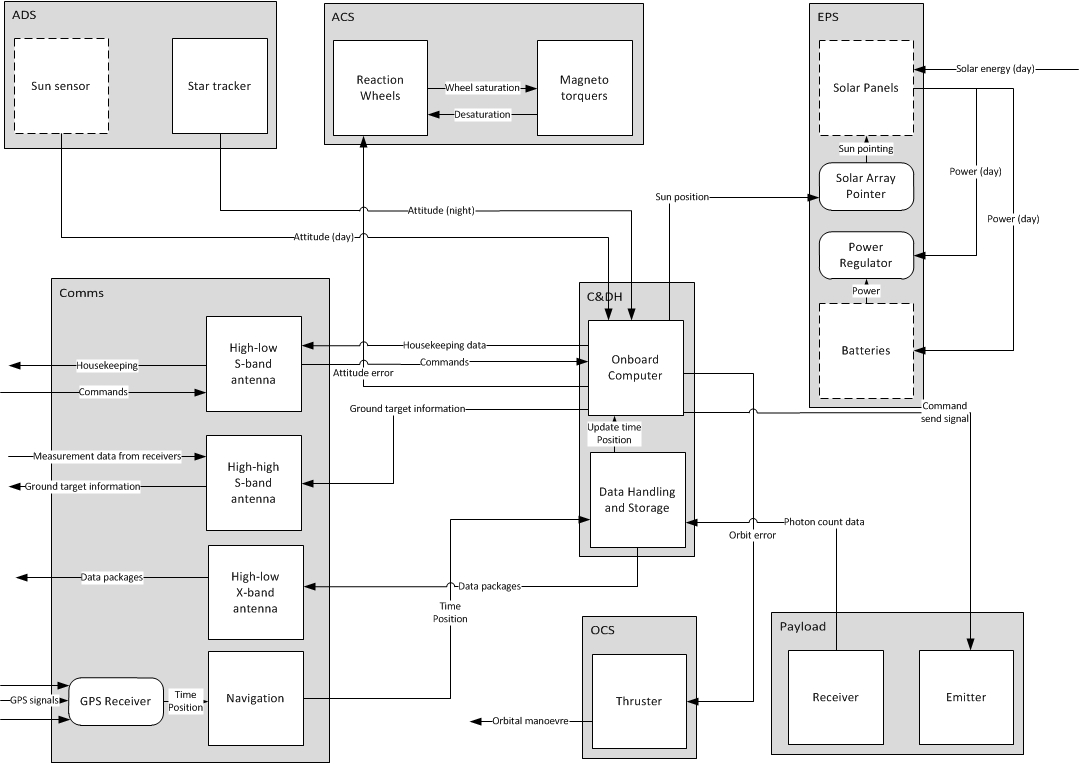
\includegraphics[width=1\textwidth, angle=90]{chapters/img/emitterHWblock.jpg}
\caption{Hardware block diagram emitter satellite}
\label{HWblockemitter}
\end{figure}

\begin{figure}
\centering
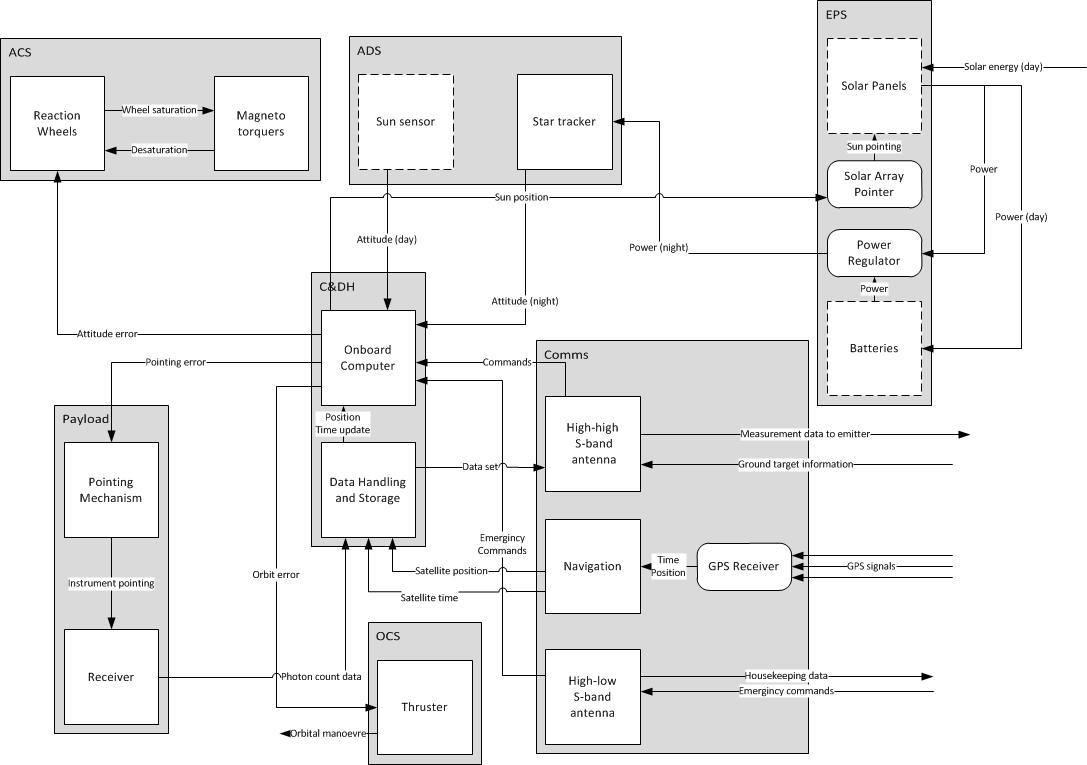
\includegraphics[width=1\textwidth, angle=90]{chapters/img/receiverHWblock.jpg}
\caption{Hardware block diagram receiver satellite}
\label{HWblockreceiver}
\end{figure}